\documentclass[11pt,A4paper,oneside]{amsart}

%\usepackage{color,graphicx}
%\usepackage{mathrsfs,amsbsy}
\usepackage{ctex}
\usepackage{amssymb}
\usepackage{amsmath}
\usepackage{amsfonts}
\usepackage{fancyhdr}
\usepackage[unicode, bookmarksnumbered]{hyperref}	% 启动超链接和 PDF 文档信息所需
\usepackage{graphicx}
\usepackage{amsthm}
\usepackage{enumerate}
\usepackage[mathscr]{eucal}
\usepackage{mathrsfs}
\usepackage{verbatim}
\usepackage{geometry}
\geometry{left=2.5cm,right=2.5cm,top=2cm,bottom=2.5cm}%具体的页边距设置
%\usepackage[notcite,notref]{showkeys}

% showkeys  make label explicit on the paper

\makeatletter
\@namedef{subjclassname@2010}{%
  \textup{2010} Mathematics Subject Classification}
\makeatother

\numberwithin{equation}{section}

\theoremstyle{plain}
\newtheorem{theorem}{Theorem}[section]
\newtheorem{lemma}[theorem]{Lemma}
\newtheorem{proposition}[theorem]{Proposition}
\newtheorem{corollary}[theorem]{Corollary}
\newtheorem{claim}[theorem]{Claim}
\newtheorem{defn}[theorem]{Definition}

\theoremstyle{plain}
\newtheorem{thmsub}{Theorem}[subsection]
\newtheorem{lemmasub}[thmsub]{Lemma}
\newtheorem{corollarysub}[thmsub]{Corollary}
\newtheorem{propositionsub}[thmsub]{Proposition}
\newtheorem{defnsub}[thmsub]{Definition}

\numberwithin{equation}{section}


\theoremstyle{remark}
\newtheorem{remark}[theorem]{Remark}
\newtheorem{remarks}{Remarks}


%\renewcommand\thefootnote{\fnsymbol{footnote}}
%dont use number as footnote symbol, use this command to change

\DeclareMathOperator{\supp}{supp}
\DeclareMathOperator{\dist}{dist}
\DeclareMathOperator{\vol}{vol}
\DeclareMathOperator{\diag}{diag}
\DeclareMathOperator{\tr}{tr}


\begin{document}

\title[]{\LARGE 拓扑学参考书籍}


\author[]{\large 周潇翔}
\address{School of Mathematical Sciences\\
University of Science and Technology of China\\
Hefei, 230026\\ P.R. China\\}
\email{xx352229@mail.ustc.edu.cn}
\maketitle




\begin{abstract}
简要地说明一下拓扑学的内容和参考书籍。
\end{abstract}




%%%%%%%%%%%%%%%%%%%%%%%%%%%%%%%%%%%%%%%%%%%%%%%%%%%%%%%%%%%%%%%%%%%%%%%%%%%%%%%%%%%%%%%%%%%%%

你们既然下学期要提前选课(或者旁听),就得提前做好准备。
\section{Tips}
一些与课程内容无关的小Tips:
\begin{enumerate}
	\item 尽可能用好英文书后的附录。英文书后往往有一些Index(术语),很多概念可以很快地从这里查阅到;另外,书后的Bibliography(参考文献)有时可以帮助你深入探索某个专题(如,\cite{MAA97}这里的参考文献有说哪本书里有什么具体的内容;)另外,在\cite[p577]{EC18}有一些关于拓扑学的评论,还有\cite[Appendix A]{JM08}的\textbf{(第二版)}是一个非常棒的拓扑学基本概念的总结练习。
	\item 同样的,选了课的同学请一定要及时交作业!(因为作业分而拉低绩点的真的是太亏了)另外一个,复习也不要拖太久。大一的同学请互帮互助,确实选高年级的课程,难度还是很大的。
\end{enumerate}



\section{简要介绍}
你可以参考:\href{http://elective.pku.edu.cn/elective2008/edu/pku/stu/elective/controller/courseDetail/getCourseDetail.do?kclx=BK&course_seq_no=BZ1819100130161_18397}{北大拓扑学课程信息}\footnote{可参见:\url{http://elective.pku.edu.cn/elective2008/edu/pku/stu/elective/controller/courseDetail/getCourseDetail.do?kclx=BK\&course\_seq\_no=BZ1819100130161\_18397}}与\href{http://www.math.pku.edu.cn/teachers/wangjj/2018fall/index.html}{主页}\footnote{可参见:\url{http://www.math.pku.edu.cn/teachers/wangjj/2018fall/index.html}}看过之后即可跳过这一节。\\
点集拓扑学也就只有两大块:拓扑的基本概念和基本群。数学中总是想区分什么是一样的,而什么是不一样的。在不同的等价关系下,这个问题有着不同的答案,而拓扑学关注的等价关系主要是\emph{同胚}与\emph{同伦}。\\
为了说明两个空间是同胚的,只需构造一个具体的同胚映射即可;而为了说明两个空间不是同胚的,我们的做法往往是寻找一个在同胚映射下的不变量(比如分离性、可数性、紧致性与列紧性、连通性与道路连通性),其中最不平凡的是基本群。如果两个空间的这些量都不相等,自然不存在这两个空间之间的同胚映射。\\
基本群是使用代数方法来研究几何的开端。你会尝试使用van Kampen定理来计算一些空间的基本群,并使用基本群来对二维闭曲面进行彻底的分类(判断两个闭曲面是否不同胚)




\section{预备知识}
\begin{itemize}
	\item $\mathbb{R}^n$中的拓扑概念,见\cite[Chapter 8]{CS12}。
    \item 群论的基本知识
\end{itemize}


\begin{figure}[!h]
	\section{推荐阅读顺序}
	\begin{minipage}[b]{.70\textwidth}
		\begin{itemize}
			\item 请先阅读\cite[Chapter 8]{CS12},请确保自己了解了$\mathbb{R}^n$中的开集、闭集、连通性与道路联通性、紧性与自列紧性(重要结论:$\mathbb{R}^n$中紧集$\Leftrightarrow$自列紧集$\Leftrightarrow$有界闭集).相关材料已经上传.
			\item \cite[Section 2,4,5 \& Chapter VI]{EC18}是一个不错的科普。(这本书的特色就在于科普,让你很愉快地了解各类概念而不去细究证明中的细节,另外喜欢从简单的例子开始讲起,平易近人)
			\item 我喜欢\cite[p73-79, p82-84, p87-102]{YCY97}。这一块的几何直观非常强,而且很漂亮,也适合寒假时做一些拓扑的小实验。
			\item \cite{ZZM99}这本书和这个课关系不是很大,但是好玩。
			\item \cite{MAA97}:这本书估计就是下学期课程的主要内容了,我粗略地翻了翻,图片十分丰富,另外应该讲到的内容都讲到了。将这一本看完再把\cite[Appendix A]{JM08}看完下学期的拓扑学就稳了。我下学期也想把这本书看了。
			\item 据说\cite{JM00}写得细而琐碎,可以适当当参考资料。
			\item \cite{AH03}:这本书这学期狠狠地虐了我一把,所以还是放上来吧,和本课程相关的估计就第一章了。另外,Allen Hatcher的\href{http://pi.math.cornell.edu/~hatcher/}{网页}\footnote{可参见:\url{http://pi.math.cornell.edu/~hatcher}}里还是有一定货的。
		\end{itemize}
	\end{minipage}
	\begin{minipage}[b]{.27\textwidth}
		\centering
		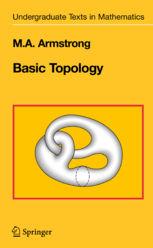
\includegraphics[width=.8\textwidth]{figures/BasicTopology.jpg}\\
		\caption{基础拓扑学}
	\end{minipage}
\end{figure}



%%%%%%%%%%%%%%%%%%%%%%%%%%%%%%%%%%%%%%%%%%%%%%%%%%%%%%%%%%%%%%%%%%%%%%%%%%%%%%%%%%%%%%%%%%%%%





%%%%%%%%%%%%%%%%%%%%%%%%%%%%%%%%%%%%%%%%%%%%%%%%%%%%%%%%%%%%%%%%%%%%%%%%%%






%%%%%%%%%%%%%%%%%%%%%%%%%%%%%%%%%%%%%%%%%%%%%%%%%%%%%%%%%%%%%%%%%%%%%%%%%%%%%%%%%%%%%%%%%%%%%%%




\begin{thebibliography}{99}


%\bibitem{AF12}%
%Antunes, P., Freitas, P.: Optimal spectral rectangles and lattice ellipses. \emph{Proc. Royal Soc. London Ser. A.} \textbf{469} (2012), 20120492.
\bibitem{MAA97}
Armstrong M A. \emph{Basic topology[J]}. Undergraduate Texts in Mathematics, 1997:137-155.
\bibitem{JM00}
James Munkres. \emph{Topology}. 2nd. Prentice-Hall, Inc., Jan. 2000. ISBN: 9788120320468
\bibitem{YCY97}%
尤承业,《基础拓扑学讲义》,北京大学出版社,1997
\bibitem{XJC81}%
熊金城,《点集拓扑讲义》,人民教育出版社,1981
\bibitem{ZZM99}%
伏·巴尔佳斯基,伏·叶弗来莫维契,裘光明. 拓扑学奇趣[J].湖南教育出版社,1999.8.
\bibitem{AH03}%
Allen Hatcher. \emph{Algebraic topology}. Cambridge, New York: Cambridge University Press, 2003. isbn: 0-521-79160-X
\bibitem{CS12}%
常庚哲,史济怀. 数学分析教程(第3版). 合肥:中国科学技术大学出版社,2012.8.
\bibitem{JM08}%
Lee J M. Introduction to smooth manifolds[M]. 2008.
\bibitem{EC18}
Evan Chen. \emph{An Infinitely Large Napkin}. draft. 2018.
URL:\href{http://web.evanchen.cc/napkin.html}{http://web.evanchen.cc/napkin.html}




\end{thebibliography}


\end{document}




